In this section, we will provide a formal analysis of the system using the Alloy language. Alloy is a lightweight formal specification language that allowed us to model the system's structure and behavior and verify the correctness of the system's design. In particular, we decided to use Alloy to provide a formal analysis of Recommendation and Interview functionalities as they are the most complex part of the system and the one that could benefit the most from a formal correctness verification.\\
In this section first, we present the code used to generate the model, divided into three main parts: signature, facts, and assertions. Each part will be thoroughly explained through comments included directly in the code. Additionally, we will provide a visual representation of the model generated by the code and its evolution over time, as the model represents a dynamic system. This will be accompanied by a brief textual explanation of the events occurring at each specific step.\\


\subsection{Signatures}
The signature part of the code defines the different entities present in the system and their relationships. In this case, we will define the main entities of S\&C such as Students, Companies, Universities, InternshipsOffer, Recommendation, and Interview. 
\lstinputlisting[language=alloy]{Latex/Alloy/Signatures.txt}

\subsection{Facts}
Facts represent the constraints that the system must respect and are always true in the model. For this application we defined numerous facts such as the necessity of a Student to have a CV to be matched with an Internship as well as the various stages of progression for an Internship Offer and Interview.
\lstinputlisting[language=alloy]{Latex/Alloy/Facts.txt}

\subsection{Assertions}
Assertions are the properties that we want to verify in the model. Such properties must hold to avoid unwanted behavior by the Platform. For this scenario we verified different aspects such as the necessity of both Student and Company to accept a Match before starting an Interview or the fact that only a Student, with a CV uploaded to the Platform, can have completed an interview.

\lstinputlisting[language=alloy]{Latex/Alloy/Assertions.txt}

\subsection{Model Visualization}
The following model was obtained with the following run:
\lstinputlisting[language=alloy]{Latex/Alloy/Run.txt}

and represent a typical evolution of the system. It is possible to see the different entities, their relationships, and the evolution of the status of some of those entities, like Recommendation or Interview, through time.\\ 
The parameters for the run command were chosen to produce a clear and readable model that is easy for the reader to understand but, they can be easily adjusted to generate a more detailed or more generalized model if a different type of analysis is required.

\begin{figure}[H]
    \hspace{-2.5cm}
    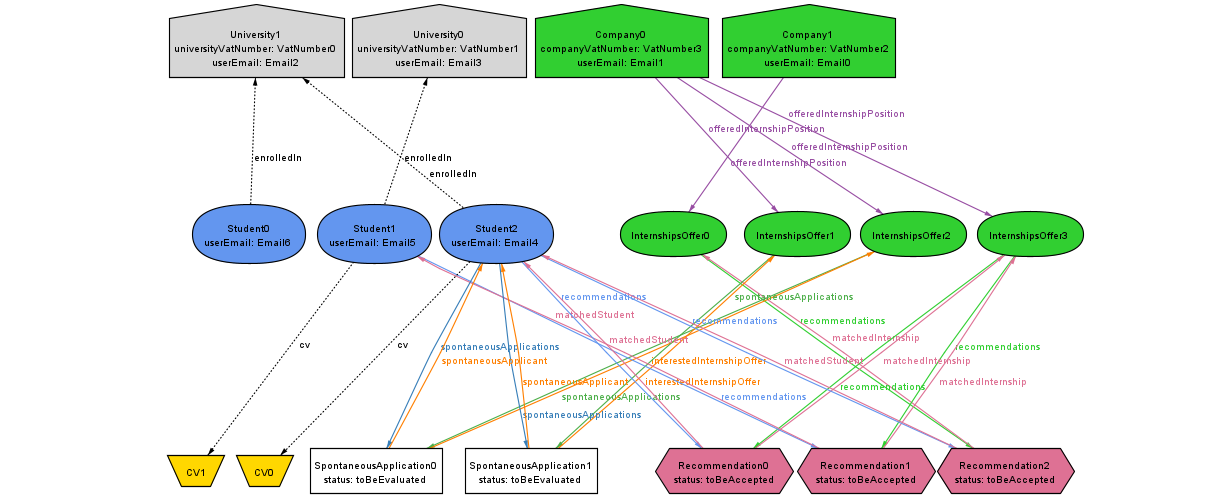
\includegraphics[width=1.3\linewidth]{Latex/Images/Alloy/0.png}
    \caption*{\textbf{Step 0:} All Recommendations and Spontaneous Applications have been sent but have not yet been evaluated. \textit{Student0} has not uploaded a CV yet, so he cannot be matched with any InternshipOffer}
    \label{fig:ALIMG0}
\end{figure}
\begin{figure}[H]
    \hspace{-2.5cm}
    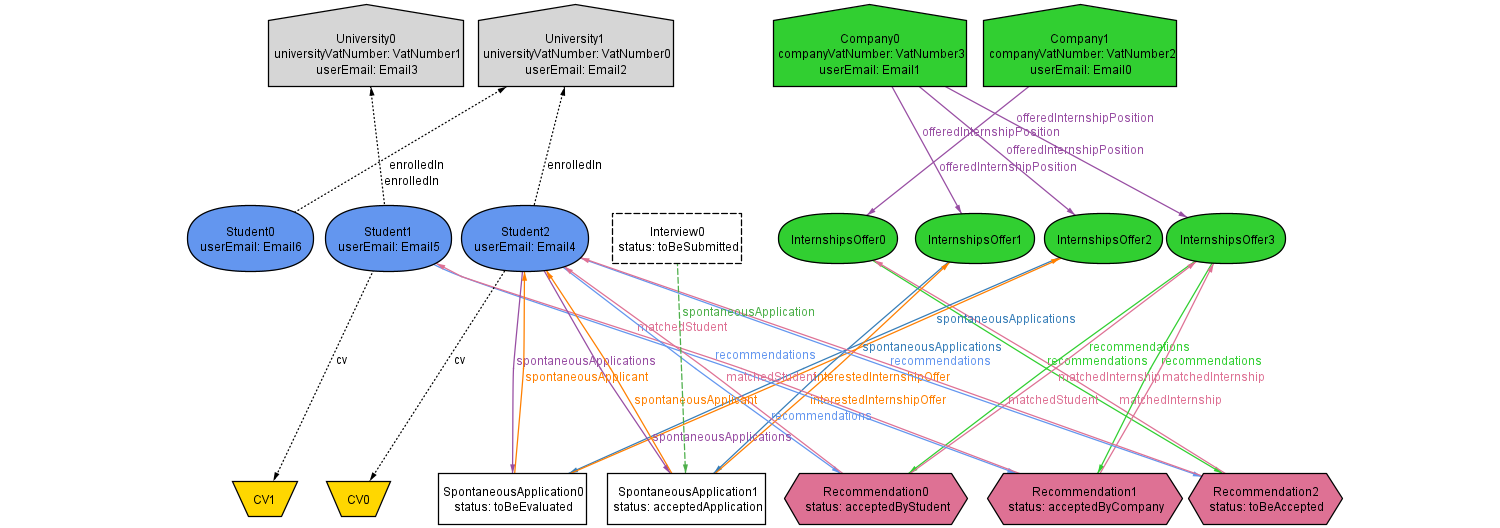
\includegraphics[width=1.3\linewidth]{Latex/Images/Alloy/1.png}
    \caption*{\textbf{Step 1:} A Spontaneous Application (\textit{SpontanousApplication1}) has been accepted and a Interview  (\textit{Interview0}) has been created}
    \label{fig:ALIMG1}
\end{figure}
\begin{figure}[H]
    \hspace{-2.5cm}
    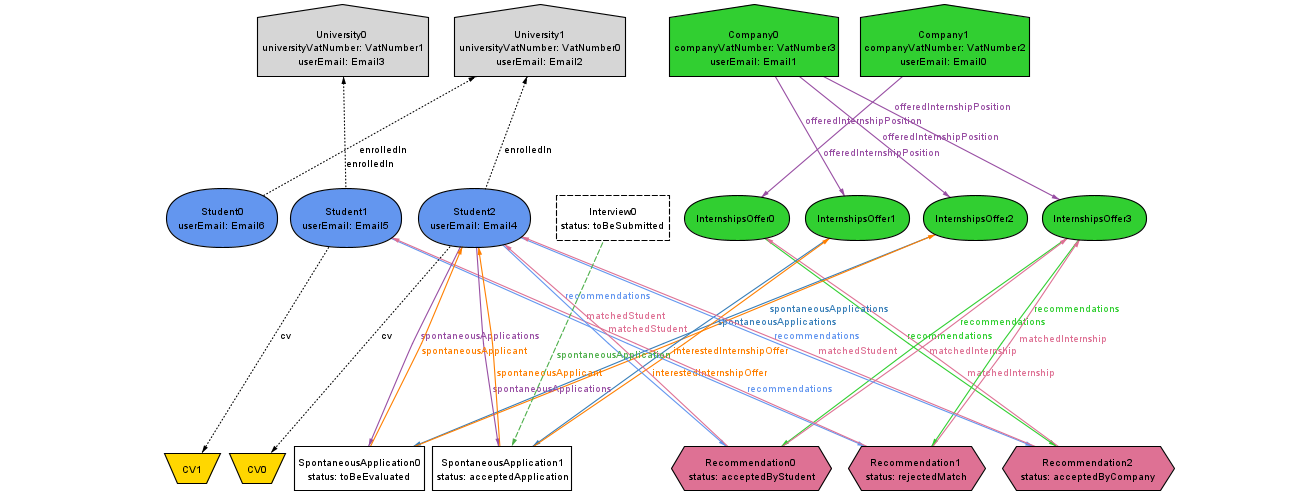
\includegraphics[width=1.3\linewidth]{Latex/Images/Alloy/2.png}
    \caption*{\textbf{Step 2:} A Recommendation (\textit{Recommendation1}) has been rejected by one of the party}
    \label{fig:ALIMG2}
\end{figure}
\begin{figure}[H]
    \hspace{-2.5cm}
    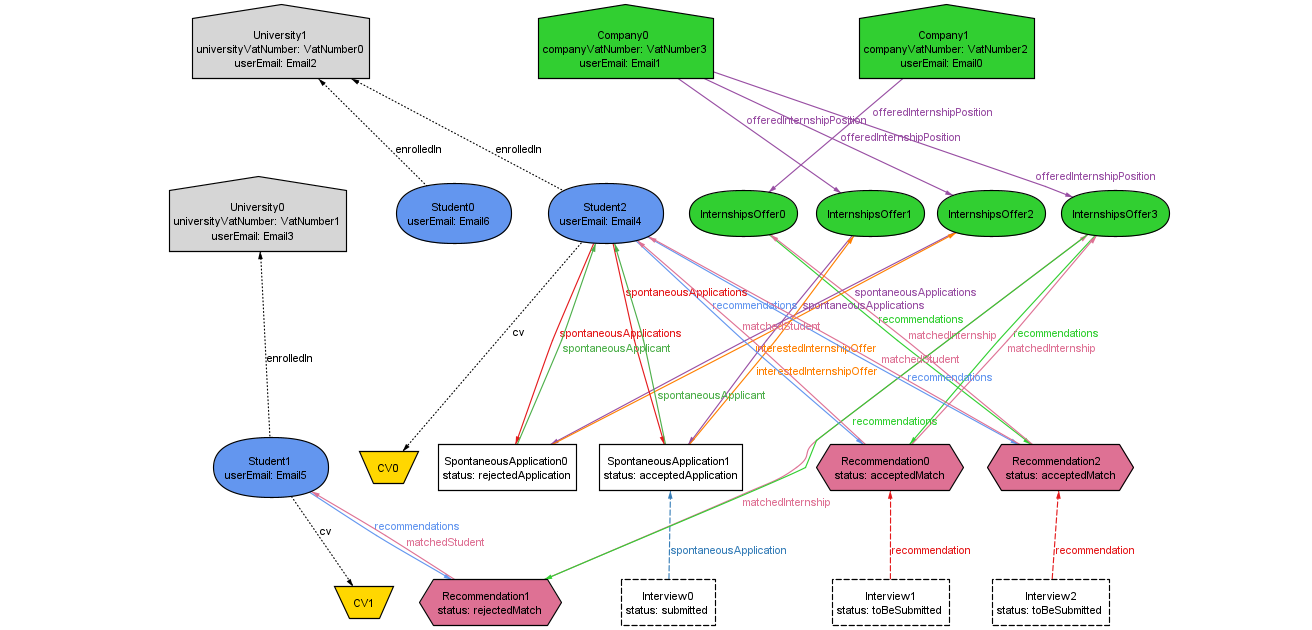
\includegraphics[width=1.3\linewidth]{Latex/Images/Alloy/3.png}
    \caption*{\textbf{Step 3:} The other Spontaneous Application (\textit{SpontanousApplication0}) has been rejected, while \textit{Interview0} has been sent. The two remaining Recommendations have been accepted by the remaining party}
    \label{fig:ALIMG3}
\end{figure}
\begin{figure}[H]
    \hspace{-2.5cm}
    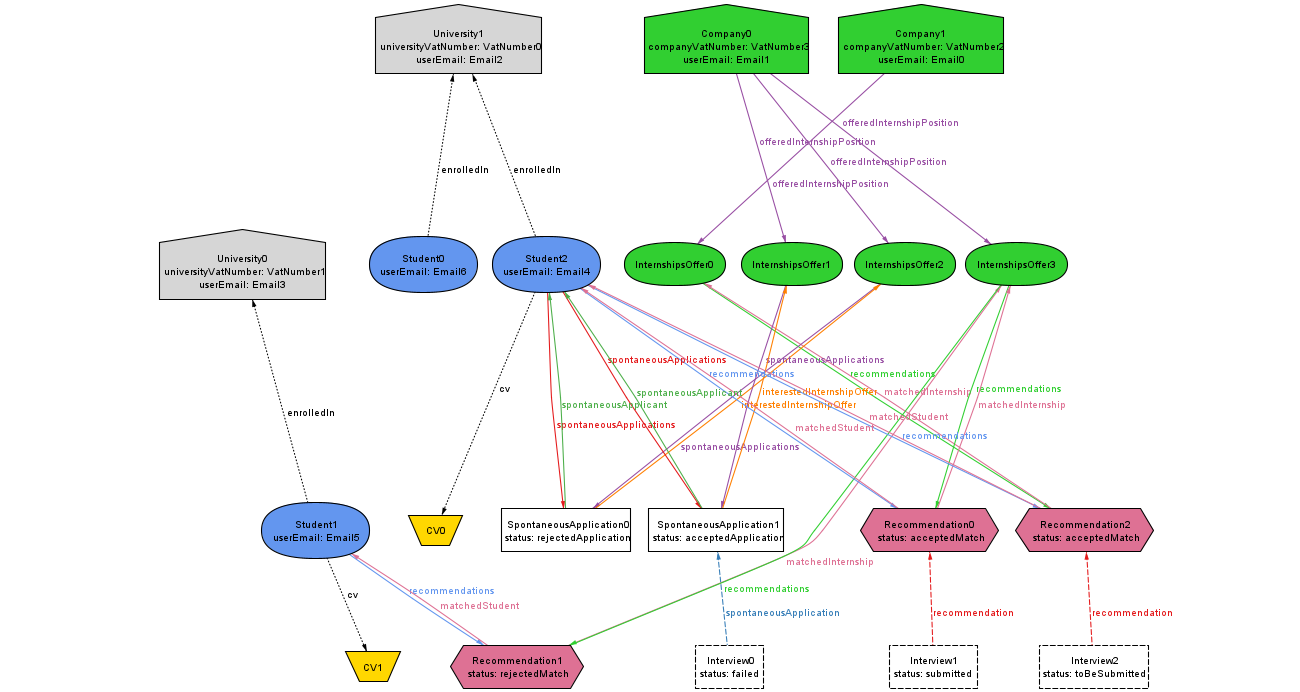
\includegraphics[width=1.3\linewidth]{Latex/Images/Alloy/4.png}
    \caption*{\textbf{Step 4:} \textit{Interview0} of \textit{Student2} was unsucesfull but Interview (\textit{Interview1}) is sent to him for another Recommendation}
    \label{fig:ALIMG4}
\end{figure}
\begin{figure}[H]
    \hspace{-2.5cm}
    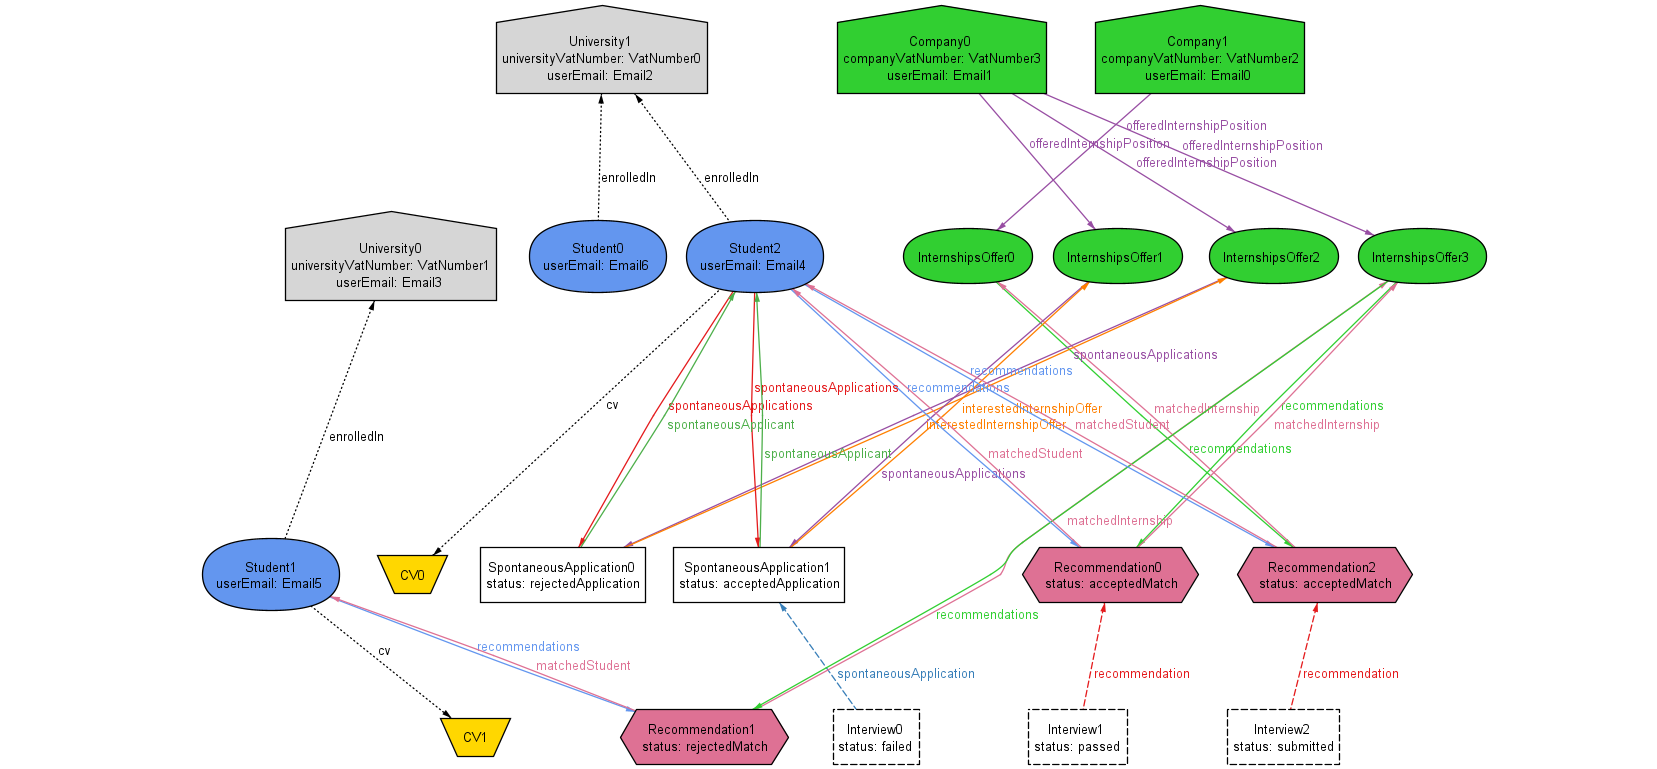
\includegraphics[width=1.3\linewidth]{Latex/Images/Alloy/5.png}
    \caption*{\textbf{Step 5:} \textit{Interview1} has been passed by \textit{Student2}, while \textit{Company1} has sent him the remaining Interview}
    \label{fig:ALIMG5}
\end{figure}


